\documentclass[a4paper,17pt]{extarticle}% packarges needed
% \usepackage[english]{babel}
\usepackage{latexsym,amssymb}
\usepackage{xcolor}
\usepackage[pdftex]{graphicx}
\usepackage{amsmath,amsfonts}
\usepackage{multicol} 
\usepackage{pifont}
\usepackage{geometry}

\usepackage{array}
\usepackage{tikz}
\usepackage{pgfplots}


%%%%%%%%%%%%%%%%%%%%%%%%%%%%%%%%%%%%%%%%%%%%%%%%%%%   adding by me %%%%%%%%%%%%%%%%%%%%%%%%%%%%%%%%%%%%%%%%

\tikzset{timed/.style=dashed}
\usetikzlibrary{shapes}
\usetikzlibrary{calc}
\usetikzlibrary{backgrounds}
\usetikzlibrary{fit}
\usetikzlibrary{patterns}

\pdfminorversion=4

\renewcommand{\refname}{\sf \large \textbf References}

% \usepackage{enumerate}

\newenvironment{thinitemize}{\itemize\addtolength{\itemsep}{-6pt}}{\enditemize}

\usepackage{paralist}
\usepackage{algorithmic}
\usepackage[plain, nothing]{algorithm}

\usepackage{empheq}
\usepackage{multirow}
\usepackage{framed}
\usepackage{fancybox}
\usepackage{wrapfig}
%\usepackage{svg}

\newenvironment{algorithmUmg}{\begin{small}\begin{tabular}{|l|}\hline}{\\ \hline \end{tabular}\end{small}}

\newcommand{\norm}[2]{\|{#1}\|_{#2}}

\newcommand{\heading}[1]{\large\textsf{\textbf{#1}}}

\newcommand{\dt}{\ensuremath{\Delta t}}
 
% graphics extensions
\DeclareGraphicsExtensions{.jpg,.pdf,.pdftex,.png}
\graphicspath{{./figures/}}
 
% parameters-
\setlength{\pdfpageheight}{594mm}
\setlength{\pdfpagewidth}{420mm}
\setlength{\paperheight}{594mm}
\setlength{\paperwidth}{420mm}
\setlength{\voffset}{-.5in}
% \setlength{\hoffset}{-1.0in}
\setlength{\hoffset}{-0.5in}
\setlength{\evensidemargin}{5mm}
\setlength{\oddsidemargin}{5mm}
\setlength{\topmargin}{0mm}
\setlength{\headheight}{0mm}
\setlength{\headsep}{0mm}
\setlength{\textheight}{624mm}
\setlength{\textwidth}{410mm}
\setlength{\parindent}{0pt}
\setlength{\parskip}{2explus2ex}
\setlength{\fboxsep}{0.01\textwidth}
\setlength{\fboxrule}{0.001\textwidth}
\newlength{\boxwidth}
\setlength{\boxwidth}{0.975\textwidth}
\setlength{\boxwidth}{0.915\textwidth}
\setlength{\columnsep}{1cm}
\setlength{\columnseprule}{0.1pt}
\setlength{\multicolsep}{0cm}
%\setcounter{unbalance}{20}


% font for titel of poster
\newcommand{\titlefont}[1]
{\protect{\fontencoding{T1}\fontfamily{pag}\fontseries{b}%
    \fontshape{n}\fontsize{1.2cm}{1ex}
    \selectfont{#1}}}

\newcommand{\subtitlefont}[1]
{\protect{\fontencoding{T1}\fontfamily{pag}%\fontseries{b}%
    \fontshape{n}\fontsize{0.9cm}{1ex}
    \selectfont{#1}}}
\newcommand{\idn}{\mbox{$1 \hspace{-1.0mm}  {\bf l}$}}

% command for page headings
\newcommand{\newpart}[1]
%{\colorbox[rgb]{0.92,0.92,1}{\makebox[0.97\columnwidth]
%{\colorbox[rgb]{0.9569,0.3,0.1882}{\makebox[0.97\columnwidth]
{\colorbox[rgb]{1.0000, 0.9020, 0.4549}{\makebox[0.97\columnwidth]
    {\rule[-1.2ex]{0pt}{3.7ex}\partfont{#1}}}\bigskip}


% font for headings of pages
\newcommand{\partfont}[1]{{\Large \textsf{\textbf{#1}}}}


% page style
\pagestyle{empty}




% -------------------------------------------------------------------------
\newcommand{\pmat}[1]{\begin{pmatrix}#1\end{pmatrix}} 
\newcommand{\red}[1]{\textcolor{red}{#1}}
\newcommand{\blue}[1]{\textcolor{blue}{#1}}
\newcommand{\brown}[1]{\textcolor{brown}{#1}}
\newcommand{\green}[1]{\textcolor{green}{#1}}
\newcommand{\purple}[1]{\textcolor{purple}{#1}}
\newcommand{\gray}[1]{\textcolor{gray}{#1}}

\newcommand{\integral}[1]{\int_{t_0}^{t_N} {#1} \, dt}
\newcommand{\fsum}[3]{\sum_{#1}^{#2}{#3}} 
\newcommand{\pder}[2]{\frac{\partial #1}{\partial #2}}
\newcommand{\dder}[2]{\frac{d #1}{d #2}}

\def \R{\bb{R}}\def \C{\bb{C}}\def \Z{\bb{Z}}\def \N{\bb{N}}
\def \a{{\bf a}}
\def \b{{\bf b}}
\def \c{{\bf c}}
\def \d{{\bf d}}
\def \e{{\bf e}}
\def \f{{\bf f}}
\def \g{{\bf g}}
\def \k{{\bf k}}
\def \m{{\bf m}}
\def \n{{\bf n}}
\def \p{{\bf p}}
\def \q{{\bf q}}
\def \r{{\bf r}}
\def \s{{\bf s}}
\def \t{{\bf t}}
\def \u{{\bf u}}
\def \v{{\bf v}}
\def \w{{\bf w}}
\def \x{{\bf x}}
\def \y{{\bf y}}
\def \h{{\bf h}}
\def \z{{\bf z}}
\def \rh{{\alert{h}}}
\def \M{{\cal M}}
\def \F{{\cal F}}
\def \L{{\cal L}}
\def \R{{\bf R}}
\def \J{{\cal J}}
\def\0{{\bf 0}}
\def\p{{\bf{g}}}
\def \blambda{{\boldsymbol{\lambda}}}
%--------------------------------------------------------------------------
%%%%%%%%%%%%%%%%%%%%%%%%%%%%%%%
%%%%%%%%%%%%%%%%%%%%%%%%%%%%%%%

\def\minim{\mathop{\hbox{\rm minimize}}}
\def\minimize#1{{\displaystyle\minim_{#1}}}
\def\subject{\mbox{\rm subject to}}
\def\myobj{J}
\def\problemI#1#2#3#4{%\fbox
   {\begin{tabular*}{0.3\textwidth}
    {@{}l@{\extracolsep{\fill}}l@{\extracolsep{6pt}}l@{\extracolsep{\fill}}c@{}}
      #1 & $\minimize{#2}$ & $#3$ & $ $ \\[5pt]
         & $\subject$      & $#4$ & $ $
    \end{tabular*}}}

\def\problemII#1#2#3#4#5{%\fbox
   {\begin{tabular*}{0.3\textwidth}
    {@{}l@{\extracolsep{\fill}}l@{\extracolsep{6pt}}l@{\extracolsep{\fill}}c@{}}
      #1 & $\minimize{#2}$ & $#3$ & $ $ \\[5pt]
         & $\subject$      & $#4$ & $ $ \\[5pt]
         & & $#5$ & $ $
    \end{tabular*}}}

\def\problemIII#1#2#3#4#5#6{%\fbox
   {\begin{tabular*}{0.3\textwidth}
    {@{}l@{\extracolsep{\fill}}l@{\extracolsep{6pt}}l@{\extracolsep{\fill}}c@{}}
      #1 & $\minimize{#2}$ & $#3$ & $ $ \\[5pt]
         & $\subject$      & $#4$ & $ $ \\[5pt]
         & & $#5$ & $ $ \\[5pt]
         & & $#6$ & $ $ 
    \end{tabular*}}}



\begin{document}


\fbox{
\parbox{0.9972\boxwidth}{

\hspace*{-.3cm}
\begin{minipage}{0.3\textwidth}
  \begin{tikzpicture}
    %\node [anchor=north] (label) at (0,0)
    %{\includegraphics[width=\textwidth]{images/eth_logo_black.pdf}};
    \node [anchor=south] (label) at (0,0.3) {
\includegraphics[width=\textwidth]{usi_logo}};
  \end{tikzpicture}
\end{minipage}
\hspace*{0.02\textheight}
\begin{minipage}{0.55\textwidth}
  \titlefont{Large Scale Xeon Phi Parallelization of a Deep Learning Language Model}\\[0.5cm]
 \subtitlefont{Tim Dettmers, Hanieh Soleimani, Olaf Schenk}
\end{minipage}
}
}

% Do not change anything in the command lines for 
% the frame box, the paragraph box or the 
% multicolumns. 


%%%%%%%%%%%%%%%%%%%%%%%%%%%%%%%%%%%%%%%%%%%%%%%%%%%%%%%%%%%%%%%%%%%%%%%%%% 
%%%%%%%%%%%%%%%%%%%%%%%%%%%%%%%%%%%%%%%%%%%%%%%%%%%%%%%%%%%%%%%%%%%%%%%%%% 

%%%%%%%%%%%%%%%%%%%%%%%%%%%%%%%%%%%%%%%%%
%
%                         R E S E R V O I R      E Q U A T I O N S
%
%%%%%%%%%%%%%%%%%%%%%%%%%%%%%%%%%%%%%%%%%

\fbox{
	\parbox{1.001\boxwidth}{
    \setlength{\fboxsep}{0.005\textwidth}
    \setlength{\fboxrule}{0.00125\textwidth}
    
    \raggedcolumns
    \begin{multicols}{2}
      
      % --------------------------------------------------------------------------
      \vbox to 0.1434\textheight {%
      \newpart{Introduction to Software Atelier Course}
      
      
          
      
               
      \begin{wrapfigure}[5]{l}{0.3\linewidth}
      \vspace{-20pt}


\includegraphics[width=.95\linewidth]{figures/usi_1.jpg} 
%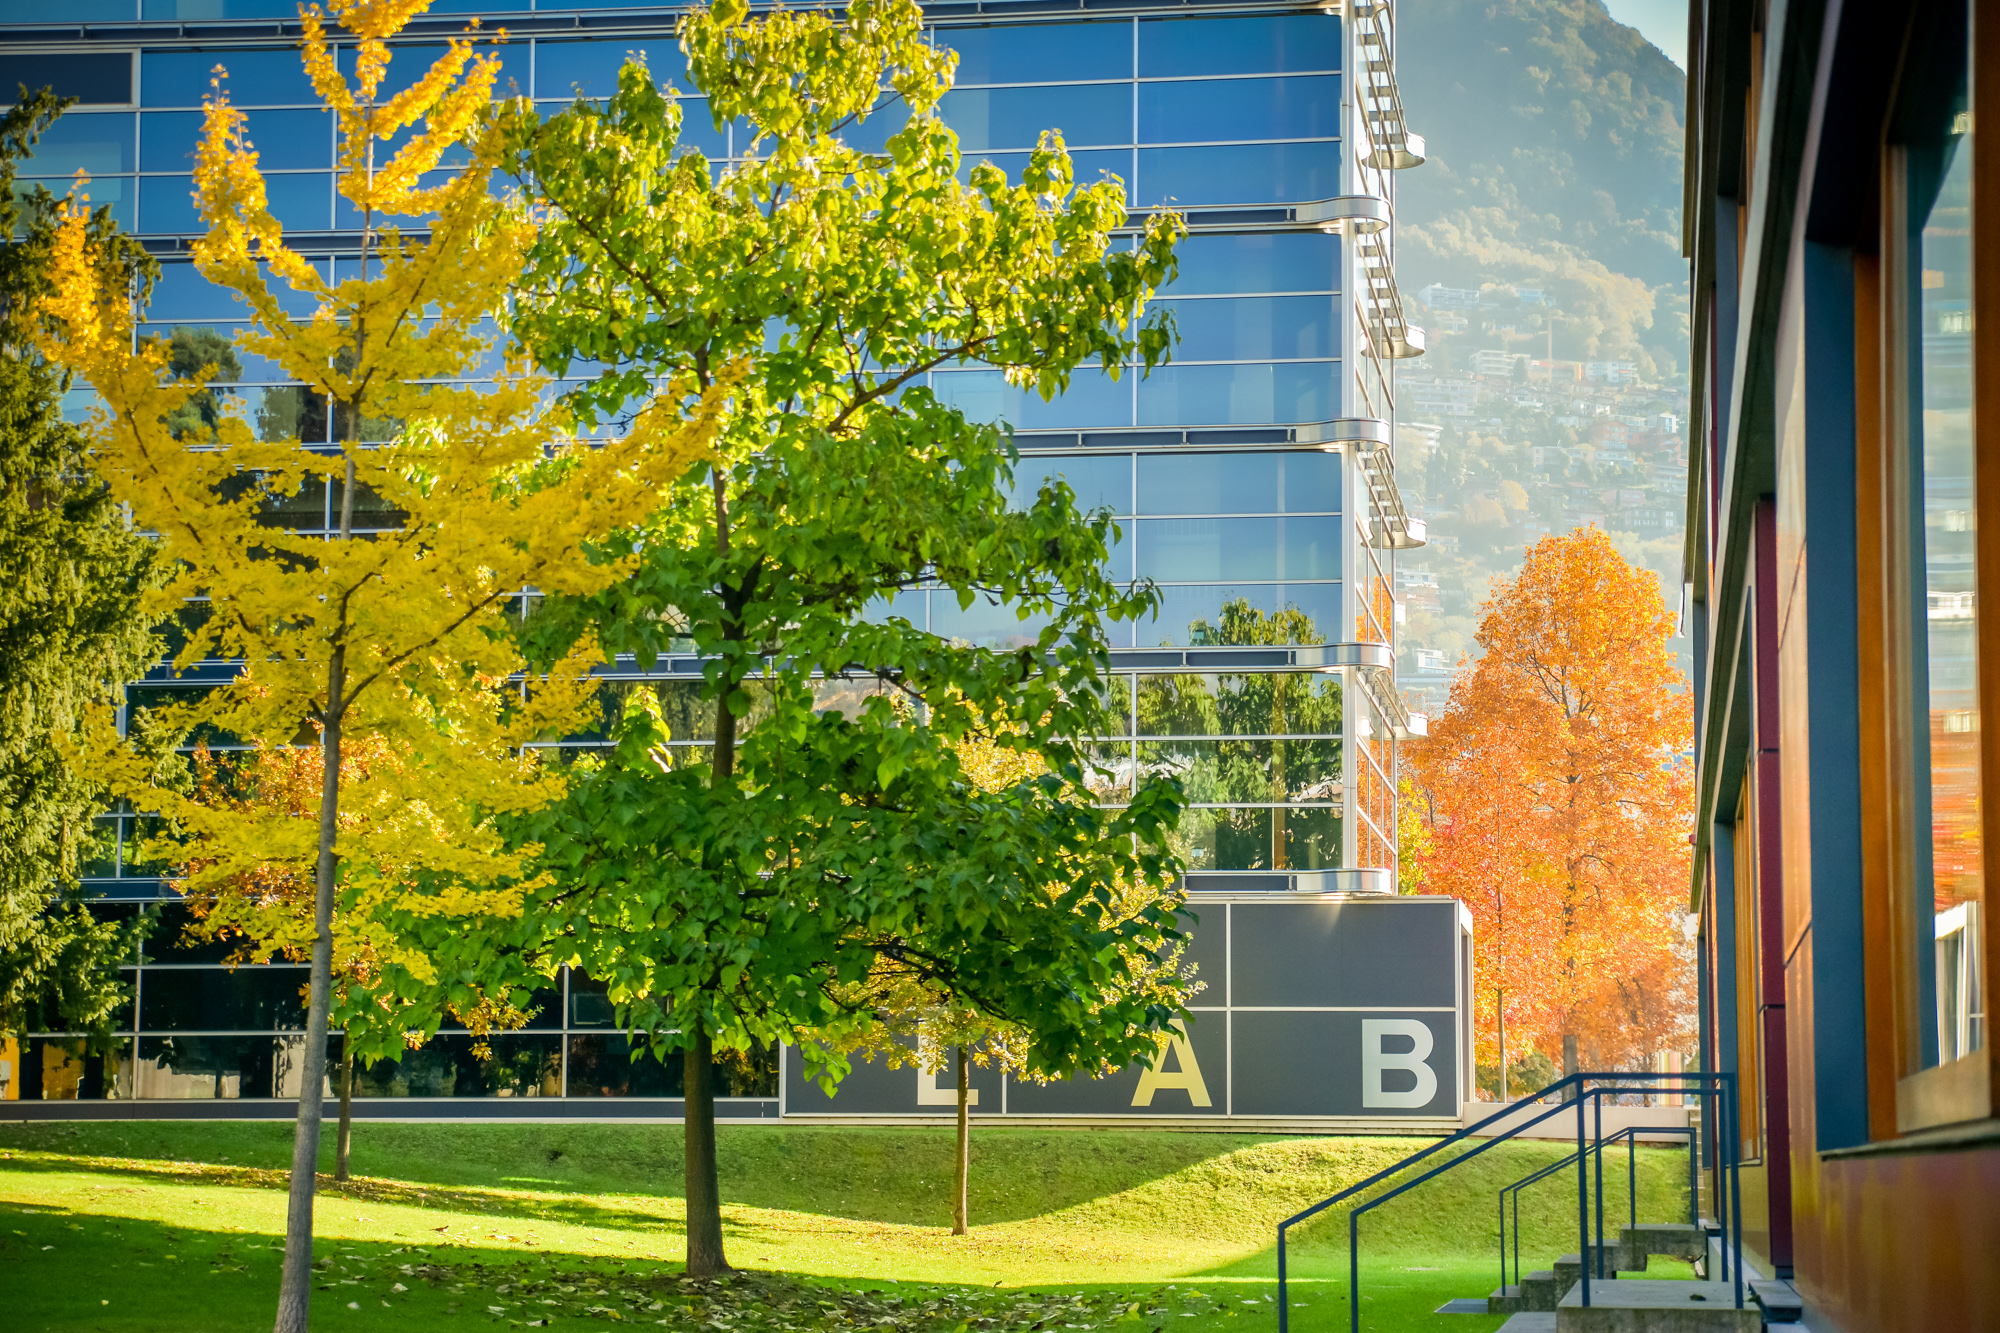
\includegraphics[width=0.48\linewidth]{figures/usi_2.jpg}

\vspace{-20pt}
\end{wrapfigure}

The Software Atelier master course at the Computational Science institute of the University of Lugano focused on the supercomputing and simulation. It was presenting advanced topics in parallel computing and numerical simulation for prospective computational and software engineers.

\begin{wrapfigure}[3]{r}{0.3\linewidth}
      \vspace{-42pt}

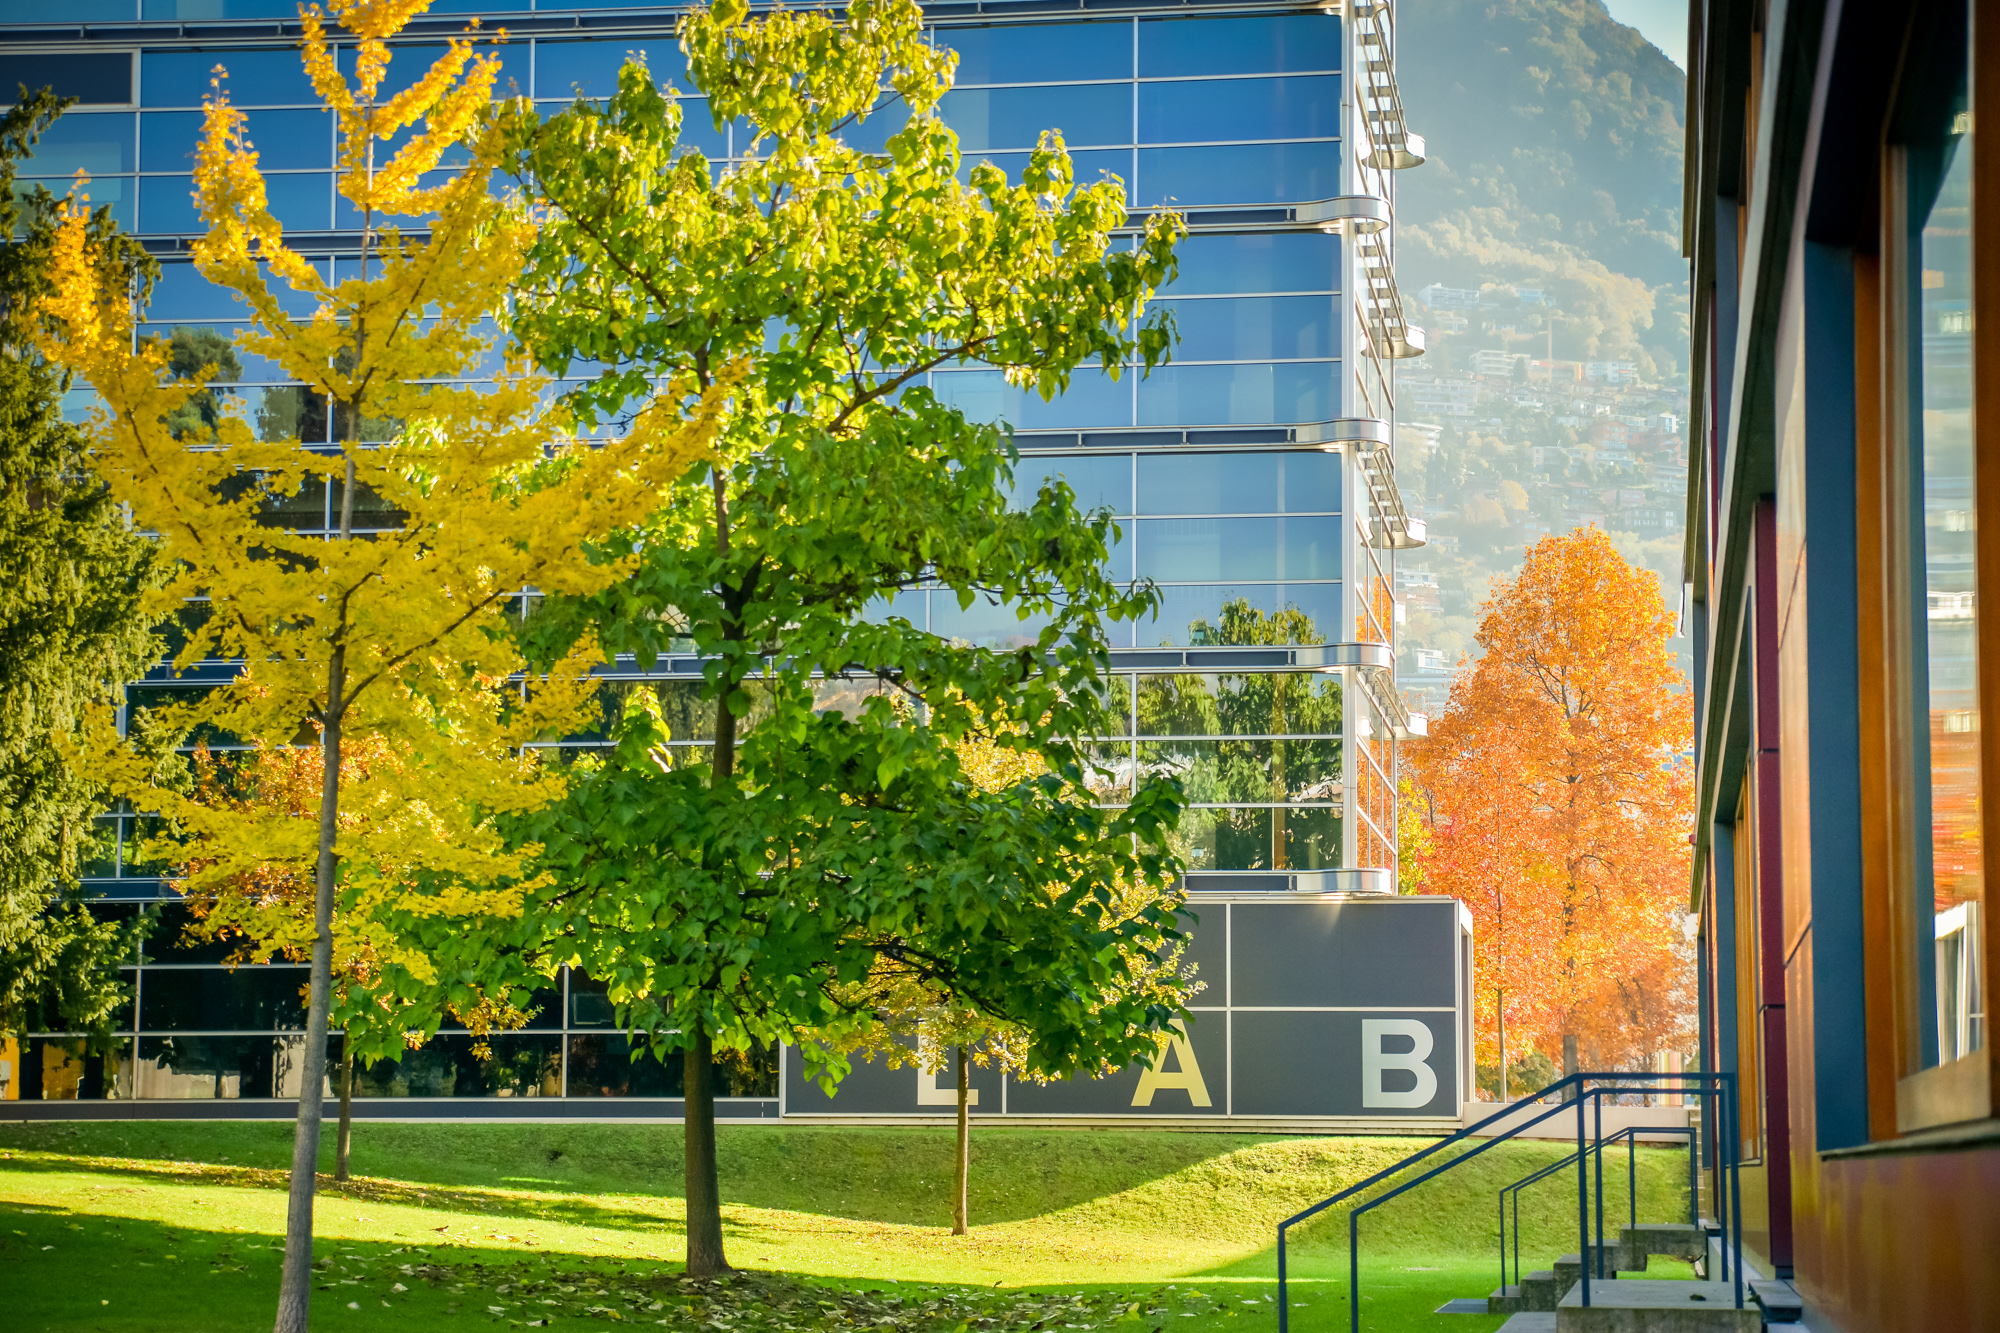
\includegraphics[width=0.95\linewidth]{figures/usi_2.jpg}

\vspace{-42pt}
\end{wrapfigure}
     

The Software Atelier master course at the Computational Science institute of the University of Lugano focused on the supercomputing and simulation.


%\vspace{-20pt}
%\end{wrapfigure}
%
%\begin{wrapfigure}{r}{0.43\linewidth}
%      \vspace{-2pt}
%      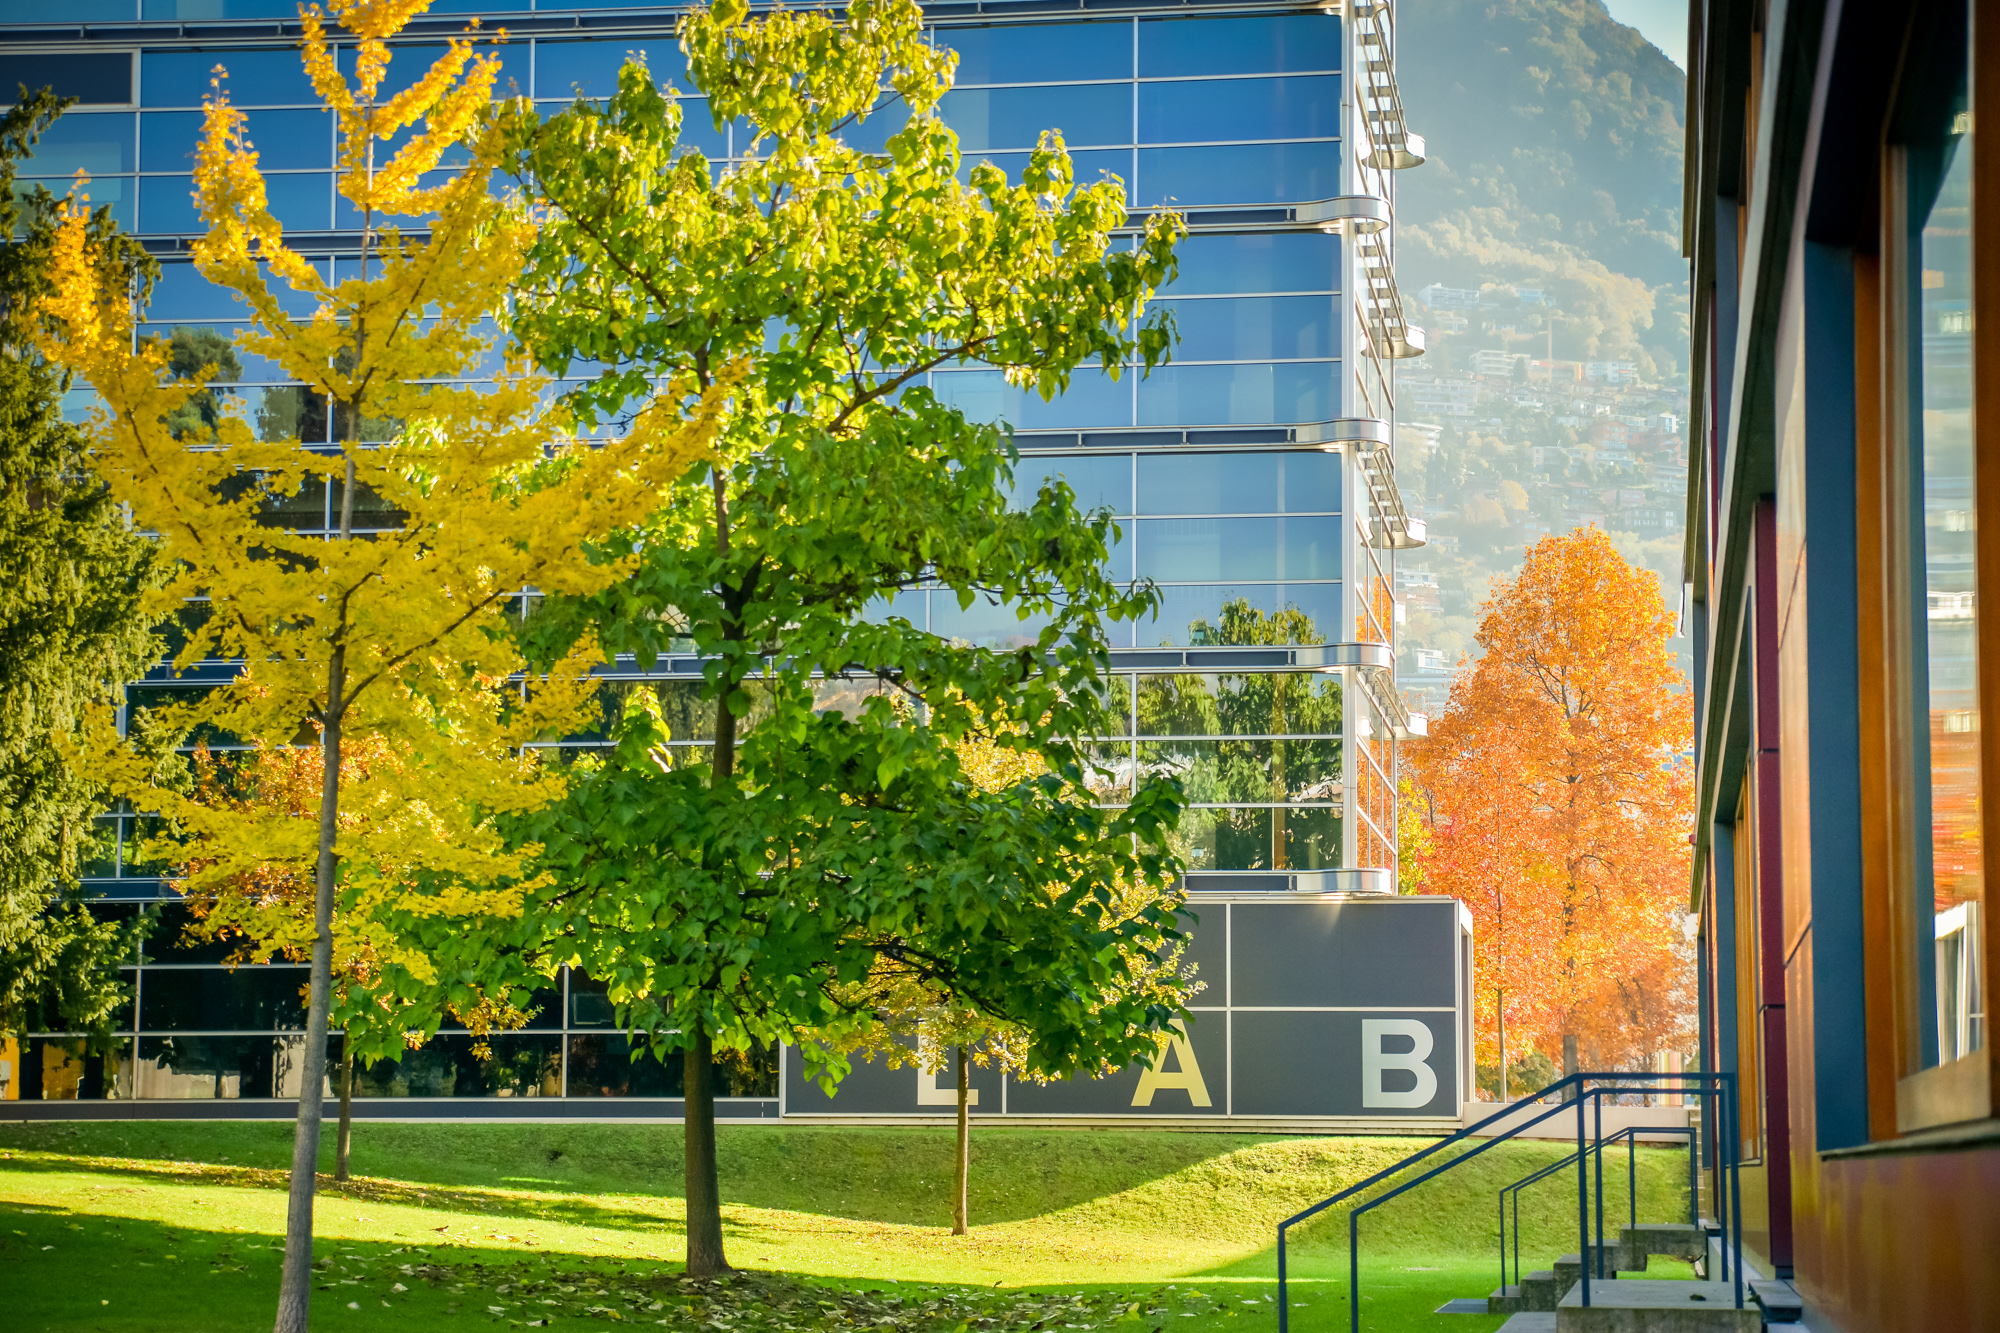
\includegraphics[width=0.95\linewidth]{figures/usi_2.jpg}
%      \vspace{-2pt}
%\end{wrapfigure}
%
%      


%\begin{tabular}{cc}
%%\includegraphics[width=0.14\textwidth]{figures/LSTM.png}
%%&
%%\includegraphics[width=0.2\textwidth]{figures/NorneSculd.jpg} %} %NorneNoLumpPieceWiseConstantPermX.png}
%%\\
%%& \\
%%{\footnotesize    
%\begin{tabular}{|c|c|c|c|}
%\hline
%Run          & (HNLP)         & (FNLP)      & (NLP)       \\
%\hline
%Ref.          & 142.0          &                  &                    \\
%1               & 146.0          &   133.9     &         153.1 \\
%2               & 143.3          &   134.7     &          149.5\\
%3               & 124.3          &   113.5     &         132.6 \\
%4               & \bf{147.8}   &   \bf{135.2}     & \bf{153.5}  \\
%5               & 146.5          &   133.3     &         146.7 \\
%6               & 146.8          &   131.9     &         139.2 \\
%7               & 146.2          &   119.3        &         150.8 \\
%8               & 146.8          &    130.2       &         149.5 \\
%9               & 146.2          &    127.5    &         135.2 \\
%\hline
%\end{tabular}
%%}
%%  \includegraphics[width=0.2\textwidth]{figures/NorneModelPermeabilityMap.png}
%% & \includegraphics[width=0.2\textwidth]{figures/NorneChart.png} \\
%% \includegraphics[width=0.2\textwidth]{figures/NorneRevenue.pdf}
%% & \includegraphics[width=0.2\textwidth]{figures/norneNoLumpImPbT300_BHP.pdf} 
% \end{tabular}
%  % footnotesize
 
%
%      (Re)Write FEM discretization in first-order form
%      \begin{equation*}
%    \frac{dy}{dt} = B y
%  \end{equation*}
%    Rewritten in integral form:
%    \begin{equation*}
%      y(t_i+\Delta t) - y(t_i) = \int_{t_i}^{t_i+\Delta t} B y(t)dt
%    \end{equation*}
%    Let $By(t)$ be approximated by Lagrange polynomial $P(t)=\sum_i^K By_i l_i(t)$ of order (K-1) to get
%    Adams-Bashforth of order K:
%    \begin{equation*}
%      y(t_i+\Delta t) = y(t_i) + \sum_{i=1}^K \alpha_iP_i,
%    \end{equation*}
%    where $P_i = By(t_i + (i-K)\Delta t)$ and $\alpha_i = \int^{\Delta
%      t}_{0}\l^{(N)}_i(t)dt$.
%
%    \begin{center}
%      \includegraphics[width=0.25\textwidth]{ab4.pdf}
%    \end{center}   
    
\vfill
%%% stop editing here
      \columnbreak
} % end vbox
%----------------------------------------------------------------------------
%\vspace{1cm}
     \columnbreak
\newpart{Intel Xeon Phi \& Salomon Cluster Overview}


\begin{wrapfigure}{r}{0.255\textwidth}
\vspace{-35pt}
\begin{center}
      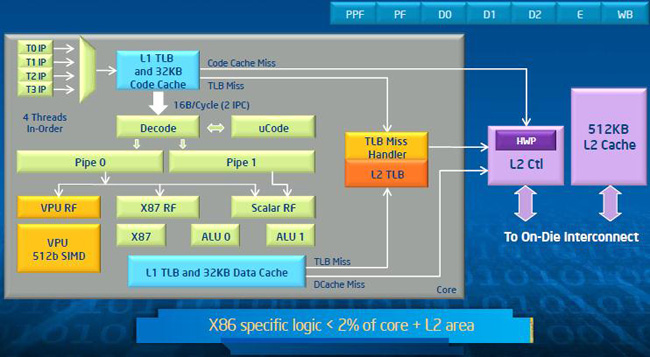
\includegraphics[width=0.252\textwidth]{figures/XeonPhi_1.jpg}
    \end{center}  
    \vspace{-35pt}
\end{wrapfigure}

Salomon Cluster has 1008 nodes, 576 of which have Xeon Phi 7120P accelerators with 2.4 TFLOPS for single precession and 352GB/s memory bandwidth. Also It has a FDR56 Infiniband interconnect which is connected in a 7D enhanced hypercube architecture     


%\begin{itemize}
%\item 1008 nodes 576 of which have Xeon Phi 7120P accelerators with 2.4 TFLOPS for single precession and 352GB/s memory bandwidth
%\item FDR56 Infiniband interconnect which is connected in a 7D enhanced hypercube architecture
%\item Total peak performance of 2011 TFLOPS
%\end{itemize}
%






%\begin{tabular}{cc}
%\includegraphics[width=0.2\textwidth]{figures/VanEssenModelPermeabilityMap.png}
%&
%\includegraphics[width=0.2\textwidth]{figures/VanEssenConstrainedDesThreshold03to1_0000.png}
%\\
% \includegraphics[width=0.2\textwidth]{figures/vanEssenRevenue.pdf}
% & \includegraphics[width=0.2\textwidth]{figures/VanEssenChart.png} \\
%  \includegraphics[width=0.2\textwidth]{figures/vanessenNoLumpIbPm_BHP.pdf}
% & \includegraphics[width=0.2\textwidth]{figures/vanessenNoLumpIbPm_BHPPrd.pdf}
% \end{tabular}
%
%%\normalsize{
%%  \begin{thebibliography}{1}
%%\bibitem{grote}\normalsize
%%{\sc M. Grote, T. Mitkova}, {\em High-order explicit local
%%  time-stepping methods for damped wave equations}, JCAM 2013
%%\bibitem{rietmann}\normalsize
%%  {\sc M. Rietmann et al.}, {\em Forward and adjoint simulations of
%%    seismic wave propagation on emerging large-scale GPU
%%    architectures}, SC 2012
%%\end{thebibliography}   
%%}
   
\end{multicols}}}

\fbox{
  \parbox{1.001\boxwidth}
  {
    \setlength{\fboxsep}{0.005\textwidth}
    \setlength{\fboxrule}{0.00125\textwidth}
    
     \raggedcolumns
      \begin{multicols}{2}
    
%%%%%%%%%%%%%%%%%%%%%%%%%%%%%%%%%%%%%%%%%
%
%                         R E S E R V O I R      E Q U A T I O N S
%
%%%%%%%%%%%%%%%%%%%%%%%%%%%%%%%%%%%%%%%%%
\vbox to 0.3234\textheight {%
 
      \newpart{Deep Learning Language Model } 



\begin{minipage}{0.33\textwidth}
	\begin{center}
		%\framebox[4.0in]{$\;$}
		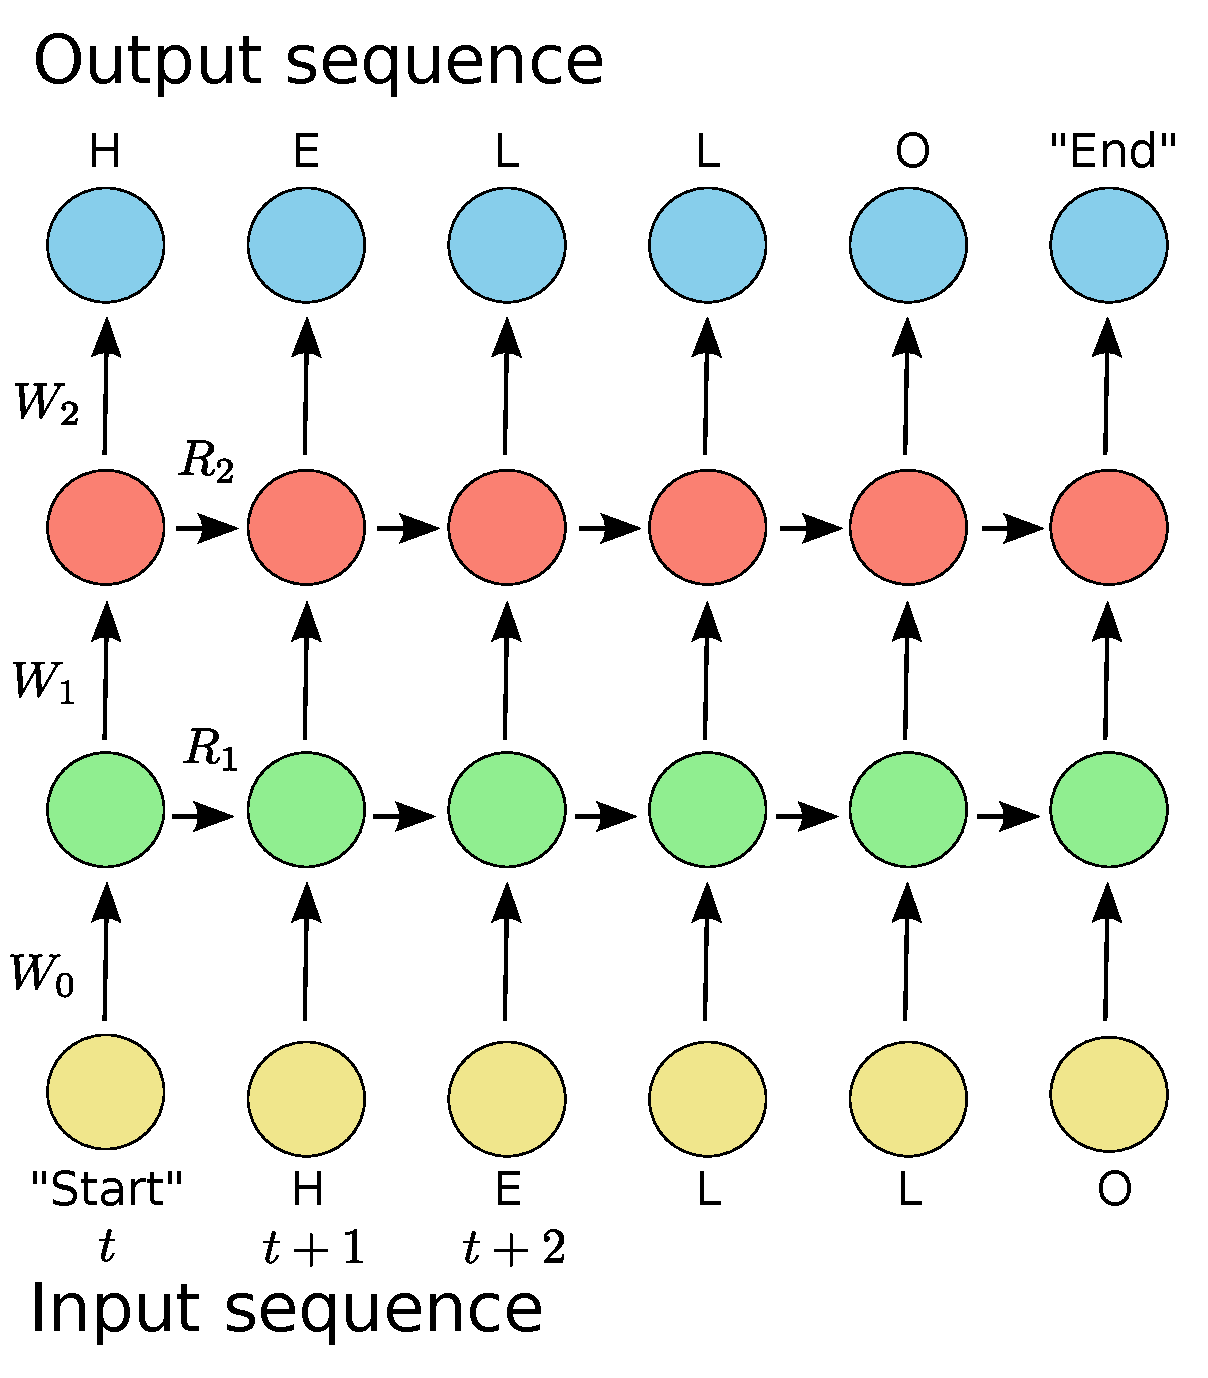
\includegraphics[width=0.6\linewidth]{figures/model.pdf}
	\end{center}
\end{minipage}

\begin{equation}
{\bf Y_{i+1}^{t+1} = A_{i}^{t}W_{i} + 
A_{i+1}^{t-1}R_{i} + B_i }
\end{equation}
\begin{equation}
{\bf A_{i+1}^{t+1} = \sigma(Y_{i+1}^{t+1}) } \end{equation}
\begin{equation}
{\bf\dfrac{\partial E}{\partial W} = \dfrac{\partial E}{\partial Y}\dfrac{\partial Y}{\partial W} = \dfrac{\partial E}{\partial A_{i+1}} \dfrac{\partial A_{i+1}}{Y}\dfrac{\partial y}{\partial W}}
\end{equation}
Here (1) and (2) are for the forward pass, (2) is the gradient for the backward pass.


} % end vbox
 \columnbreak


%%%%%%%%%%%%%%%%%%%%%%%%%%%%%%%%%%%%%%%%%
%
%                         O P T I M A L    C O N T R O L    P R O B L E M
%
%%%%%%%%%%%%%%%%%%%%%%%%%%%%%%%%%%%%%%%%%

\newpart{Results}

\begin{minipage}{0.33\textwidth}
	\begin{center}
		%\framebox[4.0in]{$\;$}
		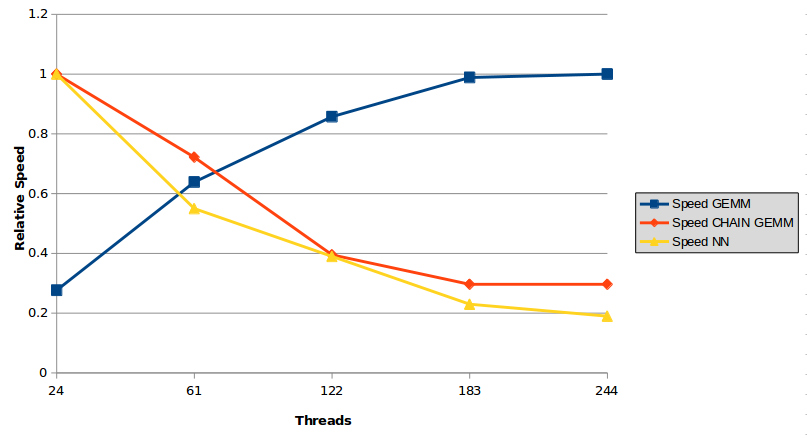
\includegraphics[width=1.3\linewidth]{figures/gemm.png}
	\end{center}
\end{minipage}

For chained small general matrix multiplications we have:
\begin{itemize}
	\item (GEMM) is fast if many threads are used (about 70\% peak performance) and slow if few threads are used (25\% of peak performance)
	\item GEMM is slow if many threads are used and the successive matrix dimensions differ (typical for a neural network; 10\% of peak performance) and faster for few threads (20\% of peak performance)
	\item It follows that neither many, nor few threads are efficient for feedforward and recurrent neural networks
	\item Random number generation on Xeon Phi for successive matrices of small size (rough size is 128x1200) is slow independent of the number of threads that are used. This decreases neural network performance by a factor of 10
\end{itemize}


\end{multicols}

   } % end parbox

} % end fbox


\fbox{
  \parbox{1.001\boxwidth}{
    \setlength{\fboxsep}{0.005\textwidth}
    \setlength{\fboxrule}{0.00125\textwidth}
    
    \raggedcolumns
    \begin{multicols}{2}
      % --------------------------------------------------------------------------
      \vbox to 0.1234\textheight {%
      \newpart{Discussion}
    
    {
%    \small  
      \begin{itemize}
	\item It is unclear what exactly causes the performance decreases for matrix operations (GEMM and random number generation) for successive matrices with different dimensions, but it has somehow to do how threads are scheduled and how resources are shared among threads.
	\item These problems made it impossible to even train a simple deep learning language model on Xeon Phi accelerators in a timely manner; the training time on one Xeon Phi would exceed one year
	\end{itemize}
	}
            
  
\vfill
%%% stop editing here
      \columnbreak
} % end vbox
%----------------------------------------------------------------------------
%\vspace{1cm}
     \columnbreak
\newpart{Future work}

\begin{itemize}
	\item Bottlenecks in GEMM and random number generation should be analyzed more carefully on both the software and hardware level
	\item Once problems with GEMM and random number generation are solved one can parallelize the deep learning language model on multiple nodes using MPI
\end{itemize}

\end{multicols}}}


	\section*{Data and code}
	\begin{itemize}
		\item  Code:https://github.com/TimDettmers/clusterNet2
		\item Data:
	\end{itemize}    



\end{document}
